\begin{figure}[htbp]
\centering
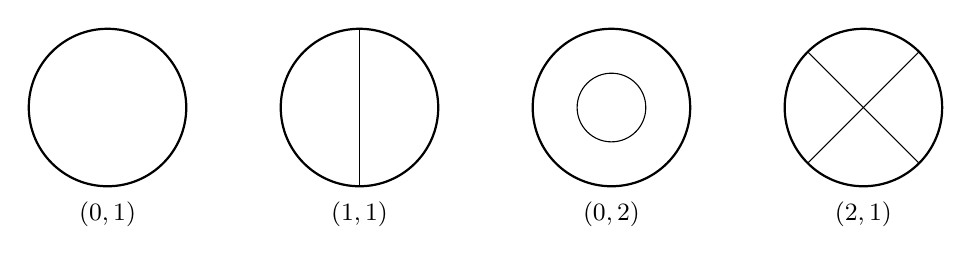
\begin{tikzpicture}[scale=1.0]
\begin{scope}
\draw[thick] (0,0) circle (1);
\node at (0,-1.35) {\small $(0,1)$};
\end{scope}
\begin{scope}[xshift=3.2cm]
\draw[thick] (0,0) circle (1);
\draw (0,-1) -- (0,1);
\node at (0,-1.35) {\small $(1,1)$};
\end{scope}
\begin{scope}[xshift=6.4cm]
\draw[thick] (0,0) circle (1);
\draw (0,0) circle (0.436);
\node at (0,-1.35) {\small $(0,2)$};
\end{scope}
\begin{scope}[xshift=9.6cm]
\draw[thick] (0,0) circle (1);
\draw (-0.707,-0.707) -- (0.707,0.707);
\draw (-0.707,0.707) -- (0.707,-0.707);
\node at (0,-1.35) {\small $(2,1)$};
\end{scope}
\end{tikzpicture}
\caption{圆膜的几个低阶模式。内部实线是节线（振动为零的线）。$(m,n)$ 中 $m$ 是节线直径数，$n-1$ 是内部节圆数；$(0,2)$ 的节圆半径按 $j_{0,1}/j_{0,2}\approx0.436$ 画出。}
\end{figure}
